\chapter{图形绘制}

科技绘图是论文中不可或缺的重要部分,信息丰富的图形一方面可以达到很好的视觉效果。另一方面,
图形辅以文字说明也能让读者更为直观地理解一些复杂的问题、过程以及结果。当论文中需要绘制一
些图形时,制作这些图形所需要花费的时间就成为影响科研进度的一个重要因素了。在日常科研工作
中,通过阅读大量文献,我们或许也会发现这样一种现象:在高质量期刊上发表学术论文,除了对论
文本身的贡献和质量有严格的把控外,通常还需要一些高质量的配图用于直观阐述一些复杂原理或者
实验结果,同时用于提高读者的阅读体验。

因此,我们应该对论文中的图形绘制引起足够的重视。如果需要,花费足够的时间和精力是值得的,
因为这既能加深自己对研究的认识和理解,也能提高审稿人和潜在读者的阅读体验。一般而言,在科
技论文中,制作图形的过程可以大致概括为:
\begin{itemize}
    \item 确定绘图内容
    \item 设计图形雏形
    \item 完善图形细节
    \item 根据内容适当调整图形
\end{itemize}

\section{基本介绍}

\emph{TikZ}宏包是在LaTeX中创建图形元素的最复杂和最强大的工具。在本节中,我们将通过一些
简单的示例来介绍如何在\emph{tikzpicture}环境中创建基本的图形元素,如:线、点、曲线、圆、矩形等。

\subsection{使用tikzpicture环境创建图形元素}

首先,我们需要通过\texttt{\textbackslash{}usepackage\{tikz\}}命令调用TikZ宏包。在绘
制图形之前,需要声明tikzpicture环境。在此我们先给出两个用TikZ绘图的例子,其后再进一步详
细介绍具体的绘图命令。

\emph{【例】}使用tikzpicture环境制作一个简单的图形:
\begin{lstlisting}[language=TeX]
    \usepackage{tikz}
    \begin{document}

    
\begin{tikzpicture}

    \draw[red,fill=red] (0,0) .. controls (0,0.75) and (-1.5,1.00) .. (-1.5,2)  arc (180:0:0.75)  -- cycle;
    \draw[red,fill=red] (0,0) .. controls (0,0.75) and ( 1.5,1.00) .. ( 1.5,2)  arc (0:180:0.75) -- cycle;

    \end{tikzpicture}
\end{lstlisting}

编译后的绘制图形如图\ref{tik:1}所示。

\begin{figure}[h]
    \centering
    
\begin{tikzpicture}
        \draw[red,fill=red] (0,0) .. controls (0,0.75) and (-1.5,1.00) .. (-1.5,2)  arc (180:0:0.75)  -- cycle;
        \draw[red,fill=red] (0,0) .. controls (0,0.75) and ( 1.5,1.00) .. ( 1.5,2)  arc (0:180:0.75) -- cycle;
    \end{tikzpicture}
    \caption{绘制后的图形}
    \label{tik:1}
\end{figure}

\emph{【例】}使用tikz宏包中的tikzpicture环境创建一个张量网络图:
\begin{lstlisting}[language=TeX]
    \documentclass[border=0.3cm, 11pt]{standalone}
    \usepackage{tikz}
    \usepackage{amsmath, amssymb, amsfonts}
    \usepackage{color}

    \begin{document}
    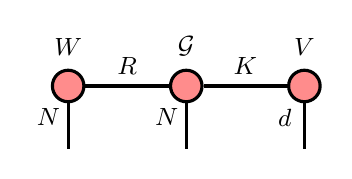
\begin{tikzpicture}

    \node[circle, line width = 0.4mm, draw = black, fill = red!45, inner sep = 0pt, minimum size = 0.4cm] (w) at (0, 0) {};
    \node at (0, 0.5) {\small{$\boldsymbol{W}$}};

    \node[circle, line width = 0.4mm, draw = black, fill = red!45, inner sep = 0pt, minimum size = 0.4cm] (g) at (1.5, 0) {};
    \node at (1.5, 0.5) {\small{$\boldsymbol{\mathcal{G}}$}};

    \node[circle, line width = 0.4mm, draw = black, fill = red!45, inner sep = 0pt, minimum size = 0.4cm] (v) at (3, 0) {};
    \node at (3, 0.5) {\small{$\boldsymbol{V}$}};

    \path [draw, line width = 0.4mm, -] (w) edge (g);
    \node at (0.75, 0.25) {\small{$R$}};
    \path [draw, line width = 0.4mm, -] (g) edge (v);
    \node at (2.25, 0.25) {\small{$K$}};

    \draw [line width = 0.4mm] (w) -- (0, -0.8);
    \node at (-0.25, -0.4) {\small{$N$}};
    \draw [line width = 0.4mm] (g) -- (1.5, -0.8);
    \node at (1.5-0.25, -0.4) {\small{$N$}};
    \draw [line width = 0.4mm] (v) -- (3, -0.8);
    \node at (3-0.25, -0.4) {\small{$d$}};

    \end{tikzpicture}
    \end{document}
\end{lstlisting}

编译后的绘制图形如图\ref{tik:2}所示。

\begin{figure}[h]
    \centering
    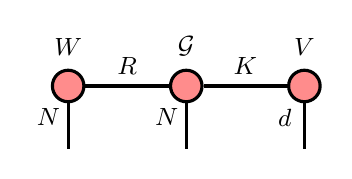
\begin{tikzpicture}
        \node[circle, line width = 0.4mm, draw = black, fill = red!45, inner sep = 0pt, minimum size = 0.4cm] (w) at (0, 0) {};
        \node at (0, 0.5) {\small{$\boldsymbol{W}$}};

        \node[circle, line width = 0.4mm, draw = black, fill = red!45, inner sep = 0pt, minimum size = 0.4cm] (g) at (1.5, 0) {};
        \node at (1.5, 0.5) {\small{$\boldsymbol{\mathcal{G}}$}};

        \node[circle, line width = 0.4mm, draw = black, fill = red!45, inner sep = 0pt, minimum size = 0.4cm] (v) at (3, 0) {};
        \node at (3, 0.5) {\small{$\boldsymbol{V}$}};

        \path [draw, line width = 0.4mm, -] (w) edge (g);
        \node at (0.75, 0.25) {\small{$R$}};
        \path [draw, line width = 0.4mm, -] (g) edge (v);
        \node at (2.25, 0.25) {\small{$K$}};

        \draw [line width = 0.4mm] (w) -- (0, -0.8);
        \node at (-0.25, -0.4) {\small{$N$}};
        \draw [line width = 0.4mm] (g) -- (1.5, -0.8);
        \node at (1.5-0.25, -0.4) {\small{$N$}};
        \draw [line width = 0.4mm] (v) -- (3, -0.8);
        \node at (3-0.25, -0.4) {\small{$d$}};
    \end{tikzpicture}
    \caption{绘制后的图形}
    \label{tik:2}
\end{figure}

\subsection{绘制直线}

我们在这两个示例中可以感受到TikZ功能的强大之处。但是,这些复杂的图形都是由最基本的点、线
和面所构成。在本小节中,我们将从绘制一条直线开始,入门这个强大的LaTeX绘图工具。首先,画
一条直线需要给出起始点坐标和终止点坐标,我们可以简单地通过如下代码:
\begin{lstlisting}[language=TeX]
    \begin{tikzpicture}
        \draw (x1,y1) -- (x2,y2); % 这里(x1,y1)和(x2,y2)在编译时均需替换成具体坐标数值。
    \end{tikzpicture}
\end{lstlisting}

来实现绘制一条从$(x1,y1)$到$(x2,y2)$的直线的功能。值得注意的是,在默认情况下,坐标系均以
cm为单位。

\emph{【例】}尝试绘制一条直线:
\begin{lstlisting}[language=TeX]
    \begin{tikzpicture}
        \draw (-2,0) -- (2,0);
    \end{tikzpicture}
\end{lstlisting}

进一步地,我们可以通过设定一系列的坐标点,来实现多条线段的连续绘制。

\emph{【例】}多条线段连续绘制:
\begin{lstlisting}[language=TeX]
    \begin{tikzpicture}
        \draw (-2,0) -- (2,0) -- (2,2) -- (-2,2) -- (-2,0);
    \end{tikzpicture}
\end{lstlisting}

也可以通过增加多行命令,实现多段线条的分开绘制。

\emph{【例】}多段线条分开绘制:
\begin{lstlisting}[language=TeX]
    \begin{tikzpicture}
        \draw (-2,0) -- (2,0) -- (2,2) -- (-2,2) -- (-2,0);
        \draw (0,4) -- (0,-2);
        \draw (3,-2) -- (3,4) -- (7,4) -- (7,-2) -- (3,-2);
        \draw (4,3) -- (6,3); \draw (4,1) -- (6,1); \draw (4,-1) -- (6,-1);
        \draw (5,3) -- (5,-1); \draw (5.75,0.25) -- (6.25,-0.25);
    \end{tikzpicture}    
\end{lstlisting}

编译后的绘制图形如图\ref{tik:3}所示。

\begin{figure}[h]
    \centering
    \begin{tikzpicture}

        \draw (-2,0) -- (2,0) -- (2,2) -- (-2,2) -- (-2,0);
        \draw (0,4) -- (0,-2);
        \draw (3,-2) -- (3,4) -- (7,4) -- (7,-2) -- (3,-2);
        \draw (4,3) -- (6,3); \draw (4,1) -- (6,1); \draw (4,-1) -- (6,-1);
        \draw (5,3) -- (5,-1); \draw (5.75,0.25) -- (6.25,-0.25);

    \end{tikzpicture}
    \caption{绘制后的图形}
    \label{tik:3}
\end{figure}

值得注意的是,在tikzpicture环境中,像\emph{Matlab}语言一样,我们需要采用\emph{;}符号来
标记一个指令的结束。这样的指令结束标记让我们不但可以在多行完成一条指令,同时也可以在一行
内实现多条指令。

\subsection{图形缩放}

在上小节中,我们绘制图形需要给出精确的坐标点。但是在绘制好之后,如果需要调整图形大小,我们
可以采用scale的方式对图形进行缩放。

\emph{【例】}整体缩放:
\begin{lstlisting}[language=TeX]
    \begin{tikzpicture}[scale=0.5]
        % 绘制内容
    \end{tikzpicture} 
\end{lstlisting}

\emph{【例】}横向缩放:
\begin{lstlisting}[language=TeX]
    \begin{tikzpicture}[xscale=1.5]
        % 绘制内容
    \end{tikzpicture} 
\end{lstlisting}

\emph{【例】}分别调整横向、纵向缩放:
\begin{lstlisting}[language=TeX]
    \begin{tikzpicture}[xscale=1.5, yscale = 2]
        % 绘制内容
    \end{tikzpicture} 
\end{lstlisting}

\subsection{绘制箭头}

在绘制直线的基础上,我们往往需要通过绘制箭头来指向性地表达意图。箭头的绘制只需要在直线绘制
的基础上,增加[option]进行声明即可。

\emph{【例】}绘制箭头:
\begin{lstlisting}[language=TeX]
    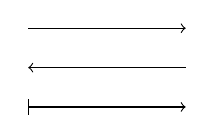
\begin{tikzpicture}

        \draw [->] (0,0) -- (2,0);
        \draw [<-] (0, -0.5) -- (2,-0.5);
        \draw [|->] (0,-1) -- (2,-1);
    
    \end{tikzpicture}
\end{lstlisting}

编译后的绘制图形如图\ref{tik:4}所示。

\begin{figure}[h]
    \centering
    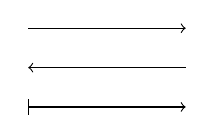
\begin{tikzpicture}

        \draw [->] (0,0) -- (2,0);
        \draw [<-] (0, -0.5) -- (2,-0.5);
        \draw [|->] (0,-1) -- (2,-1);

    \end{tikzpicture}
    \caption{绘制后的图形}
    \label{tik:4}
\end{figure}

\emph{【例】}利用绘制箭头的例子以及多条线段连续绘制的例子,用一行命令绘制一个直角坐标系:
\begin{lstlisting}[language=TeX]
    \begin{tikzpicture}

        \draw [<->] (0,2) -- (0,0) -- (3,0);
    
    \end{tikzpicture}
\end{lstlisting}

编译后的绘制图形如图\ref{tik:5}所示。

\begin{figure}[h]
    \centering
    \begin{tikzpicture}

        \draw [<->] (0,2) -- (0,0) -- (3,0);

    \end{tikzpicture}
    \caption{绘制后的图形}
    \label{tik:5}
\end{figure}

\subsection{调整线条粗细}

采用\texttt{\textbackslash{}draw}命令时,增加的[option]声明也可以用来调整线条的粗细。

\emph{【例】}绘制不同粗细的线条:
\begin{lstlisting}[language=TeX]
    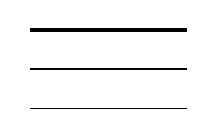
\begin{tikzpicture}

        \draw [ultra thick] (0,1) -- (2,1);
        \draw [thick] (0,0.5) -- (2,0.5);
        \draw [thin] (0,0) -- (2,0);
    
    \end{tikzpicture}
\end{lstlisting}

编译后的绘制图形如图\ref{tik:6}所示。

\begin{figure}[h]
    \centering
    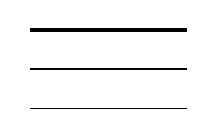
\begin{tikzpicture}

        \draw [ultra thick] (0,1) -- (2,1);
        \draw [thick] (0,0.5) -- (2,0.5);
        \draw [thin] (0,0) -- (2,0);

    \end{tikzpicture}
    \caption{绘制后的图形}
    \label{tik:6}
\end{figure}

其中,线条的粗细可以通过不同的指令来控制,从细到粗分别可调用:\emph{ultra thin},\emph{very thin},
\emph{thin},\emph{semithick},\emph{thick},\emph{very thick},\emph{ultra thick}。

\emph{【例】}绘制上述七种不同粗细的线条:
\begin{lstlisting}[language=TeX]
    
\begin{tikzpicture}

        \draw [ultra thin] (0,0) -- (2,0);
        \draw [very thin] (0,0.5) -- (2,0.5);
        \draw [thin] (0,1) -- (2,1);
        \draw [semithick] (0,1.5) -- (2,1.5);
        \draw [thick] (0,2) -- (2,2);
        \draw [very thick] (0,2.5) -- (2,2.5);
        \draw [ultra thick] (0,3) -- (2,3);
    
    \end{tikzpicture}
\end{lstlisting}

编译后的绘制图形如图\ref{tik:7}所示。

\begin{figure}[h]
    \centering
    
\begin{tikzpicture}

        \draw [ultra thin] (0,0) -- (2,0);
        \draw [very thin] (0,0.5) -- (2,0.5);
        \draw [thin] (0,1) -- (2,1);
        \draw [semithick] (0,1.5) -- (2,1.5);
        \draw [thick] (0,2) -- (2,2);
        \draw [very thick] (0,2.5) -- (2,2.5);
        \draw [ultra thick] (0,3) -- (2,3);

    \end{tikzpicture}
    \caption{绘制后的图形}
    \label{tik:7}
\end{figure}

除此之外,我们也可以自行定义线条的粗细,如[line width=5]、[line width=0.2cm]。值得注意
的是,当我们直接声明数值而不声明单位时,其默认单位均为pt。

\emph{【例】}使用line width参数绘制不同粗细线条:
\begin{lstlisting}[language=TeX]
    
\begin{tikzpicture}
        \draw [line width=3] (0,0) -- (2,0);
        \draw [line width=0.2cm] (0,0.5) -- (2,0.5);
    \end{tikzpicture}
\end{lstlisting}

编译后的绘制图形如图\ref{tik:8}所示。

\begin{figure}[h]
    \centering
    
\begin{tikzpicture}

        \draw [line width=3] (0,0) -- (2,0);
        \draw [line width=0.2cm] (0,0.5) -- (2,0.5);

    \end{tikzpicture}
    \caption{绘制后的图形}
    \label{tik:8}
\end{figure}

\subsection{虚线}

我们也可以在[option]声明中增加对于线条形状的定义。如虚线\emph{dashed}和点线\emph{dotted}。

\emph{【例】}绘制虚线:
\begin{lstlisting}[language=TeX]
    \begin{tikzpicture}

        \draw [dashed, ultra thick] (0,1) -- (2,1); %我们可以通过组合多种option来声明线条的多种特征。
        \draw [dashed] (0, 0.5) -- (2,0.5);
        \draw [dotted] (0,0) -- (2,0);
    
    \end{tikzpicture}
\end{lstlisting}

编译后的绘制图形如图\ref{tik:9}所示。

\begin{figure}[h]
    \centering
    \begin{tikzpicture}

        \draw [dashed, ultra thick] (0,1) -- (2,1); %我们可以通过组合多种option来声明线条的多种特征。
        \draw [dashed] (0, 0.5) -- (2,0.5);
        \draw [dotted] (0,0) -- (2,0);

    \end{tikzpicture}
    \caption{绘制后的图形}
    \label{tik:9}
\end{figure}

\subsection{颜色}

我们也可以在[option]声明中增加对于线条颜色的定义。如红色\emph{red}、 绿色\emph{green}、蓝色\emph{blue}等等。

\emph{【例】}绘制不同颜色的直线:
\begin{lstlisting}[language=TeX]
    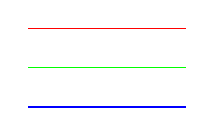
\begin{tikzpicture}

        \draw [red] (0,1) -- (2,1);
        \draw [green] (0, 0.5) -- (2,0.5);
        \draw [blue] (0,0) -- (2,0);
    
    \end{tikzpicture}
\end{lstlisting}

编译后的绘制图形如图\ref{tik:10}所示。

\begin{figure}[h]
    \centering
    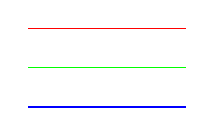
\begin{tikzpicture}

        \draw [red] (0,1) -- (2,1);
        \draw [green] (0, 0.5) -- (2,0.5);
        \draw [blue] (0,0) -- (2,0);

    \end{tikzpicture}
    \caption{绘制后的图形}
    \label{tik:10}
\end{figure}